%%%%%%%%%%%%%%%%%%%%%%%%%%%%%%%%%%%%%%%%%
% Beamer Presentation
% LaTeX Template
% Version 1.0 (10/11/12)
%
% This template has been downloaded from:
% http://www.LaTeXTemplates.com
%
% License:
% CC BY-NC-SA 3.0 (http://creativecommons.org/licenses/by-nc-sa/3.0/)
%
%%%%%%%%%%%%%%%%%%%%%%%%%%%%%%%%%%%%%%%%%

%----------------------------------------------------------------------------------------
%	PACKAGES AND THEMES
%----------------------------------------------------------------------------------------

\documentclass{beamer}

\mode<presentation> {

% The Beamer class comes with a number of default slide themes
% which change the colors and layouts of slides. Below this is a list
% of all the themes, uncomment each in turn to see what they look like.

%\usetheme{default}
%\usetheme{AnnArbor}
%\usetheme{Antibes}
%\usetheme{Bergen}
%\usetheme{Berkeley}
%\usetheme{Berlin}
%\usetheme{Boadilla}
%\usetheme{CambridgeUS}
%\usetheme{Copenhagen}
%\usetheme{Darmstadt}
%\usetheme{Dresden}
%\usetheme{Frankfurt}
%\usetheme{Goettingen}
%\usetheme{Hannover}
%\usetheme{Ilmenau}
%\usetheme{JuanLesPins}
%\usetheme{Luebeck}
\usetheme{Madrid}
%\usetheme{Malmoe}
%\usetheme{Marburg}
%\usetheme{Montpellier}
%\usetheme{PaloAlto}
%\usetheme{Pittsburgh}
%\usetheme{Rochester}
%\usetheme{Singapore}
%\usetheme{Szeged}
%\usetheme{Warsaw}

% As well as themes, the Beamer class has a number of color themes
% for any slide theme. Uncomment each of these in turn to see how it
% changes the colors of your current slide theme.

%\usecolortheme{albatross}
%\usecolortheme{beaver}
%\usecolortheme{beetle}
%\usecolortheme{crane}
%\usecolortheme{dolphin}
%\usecolortheme{dove}
%\usecolortheme{fly}
%\usecolortheme{lily}
%\usecolortheme{orchid}
%\usecolortheme{rose}
%\usecolortheme{seagull}
%\usecolortheme{seahorse}
%\usecolortheme{whale}
%\usecolortheme{wolverine}

%\setbeamertemplate{footline} % To remove the footer line in all slides uncomment this line
%\setbeamertemplate{footline}[page number] % To replace the footer line in all slides with a simple slide count uncomment this line

\setbeamertemplate{navigation symbols}{} % To remove the navigation symbols from the bottom of all slides uncomment this line
}

\usepackage{graphicx} % Allows including images
%\usepackage{booktabs} % Allows the use of \toprule, \midrule and
                      % \bottomrule in tables
\usepackage{tikz}
\usepackage{tikz-cd}
\usepackage{varwidth}
\usepackage{amsmath}
\usepackage[author-year]{amsrefs}
\usepackage{../ReAdTeX/readtex-core}
% \usepackage{../ReAdTeX/readtex-dangerous}
% \usepackage{../ReAdTeX/readtex-abstract-algebra}
\usepackage{ytableau}
\usepackage{hyperref}
%%%%%%%%%%%%%%%%%%%%%%%%%%%%%%%%%%%%%%%%%%%%%%%%%%%%%%%%%%%%%%%%%%% 
%%  MACRO DEFINITIONS:  Co-authors -- PLEASE use these! 
%%%%%%%%%%%%%%%%%%%%%%%%%%%%%%%%%%%%%%%%%%%%%%%%%%%%%%%%%%%%%%%%%%%
\definecolor{coralred}{rgb}{1.0, 0.25, 0.25}
\definecolor{lightblue}{rgb}{.3,.65,1.0} %
\DeclareMathOperator{\Gr}{Gr}
\newcommand{\cupprod}{\cup}
\newcommand{\sym}{\Lambda}
\newcommand{\lowers}{\mathcal{L}}
\newcommand{\mynone}{\ }
\newcommand{\G}{\mathfrak{G}}
\renewcommand{\S}{\mathfrak{S}}
\DeclareMathOperator{\SSYT}{SSYT}
\renewcommand{\Span}{\operatorname{sp}}
\DeclareMathOperator{\area}{area}
\DeclareMathOperator{\dinv}{dinv}
\newcommand{\DP}{\mathbf{DP}}
\newcommand{\Dyck}{\DP}
\newcommand{\PF}{\mathbf{PF}}
\newcommand{\LD}{LD}
\newcommand{\Gcal}{\mathcal{G}}
\newcommand{\Lcal}{{\mathcal L}}
\newcommand{\Ecal}{{\mathcal E}}
\newcommand{\Hbold}{{\mathbf H}}
\newcommand{\bb}{{\mathbf b}}
\newcommand{\aA}{{\mathbf a}}
\newcommand{\kk}{{\mathbf k}}
\DeclareMathOperator{\wt}{wt}
\DeclareMathOperator{\pol}{pol}


%%%%%%%%%%%%%%%%%%%%%%%%%%%%%%%%%%%%%%%%%%%%%%%%%%%%%%%%%%%%%%%%%%%% 


%----------------------------------------------------------------------------------------
%	TITLE PAGE
%----------------------------------------------------------------------------------------

\title[Shuffle Theorems]{Diagonal Harmonics and Shuffle Theorems} % The short title appears at the bottom of every slide, the full title is only on the title page

\author[George H. Seelinger]{George H. Seelinger} % Your name
\institute[UVA] % Your institution as it will appear on the bottom of every slide, may be shorthand to save space
{
  \medskip
\textit{ghs9ae@virginia.edu}\\ % Your email address
\medskip
UVA Graduate Seminar % Your institution for the title page
}
\date{29 March 2021} % Date, can be changed to a custom date
\begin{document}
\begin{frame}
 \titlepage 
\end{frame}
\begin{frame}
  \frametitle{Outline}
  \begin{enumerate}
  \item Symmetric functions, \(S_n\)-representations, and Frobenius characteristic
  \item Diagonal harmonics and shuffle conjectures
  \item Stable series approach
  \item Application: extended Delta conjecture
  \end{enumerate}\pause
  Based off of slides from
  \begin{itemize}
  \item Mark Haiman: ``A Shuffle Theorem for Paths Under Any Line''\\
    \url{https://www.math.uwaterloo.ca/~opecheni/2020-06-12-AlCoVE.pdf}
  \item Jennifer Morse: ``Hey Series, Tell Me About the Extended Delta
    Conjecture'' (ICERM, March 22, 2021)
  \end{itemize}
\end{frame}
\begin{frame}{Multivariate Polynomials}
  \begin{itemize}
  \item \(f \in \Q[x_1,\ldots,x_n]\) multivariate polynomial \pause
  \item \(\sigma \in S_n\) acts as \(\sigma.f(x_1,x_2,\ldots,x_n) =
    f(x_{\sigma(1)}, x_{\sigma(2)},\ldots,x_{\sigma(n)})\)
    \[
      \left(
        \begin{matrix}
          1 & 2 & 3\\
          3 & 2 & 1
        \end{matrix}
      \right) (5x_1^2+5x_2^2+8x_3^2) = 8x_1^2+5x_2^2+5x_3^2
    \]
  \end{itemize}
\end{frame}
\begin{frame}{Symmetric Polynomials}
  \begin{itemize}
    \item Polynomials \(f \in \Q[x_1,\ldots,x_n]\) satisfying \(\sigma.f
    = f\)? \pause
  \item Symmetric polynomials (\(n=3\))
    \begin{align*}
      e_1 = x_1 + x_2 + x_3 = & h_1  \\
      e_2 = x_1 x_2 + x_1 x_3 + x_2 x_3 \quad & h_2 = x_1^2 + x_1 x_2 + x_1
                                          x_3 + x_2^2 +  x_2 x_3 +x_3^2  \\
      e_3 = x_1 x_2 x_3 \quad & h_3 = x_1^3 + x_1^2 x_2 + x_1^2 x_3 + x_1
                          x_2^2 + \cdots
    \end{align*} \pause
  \item \(\{f \in \Q[x_1,\ldots,x_n] \st \sigma.f = f \, \forall \sigma
    \in S_n\}\) forms a vector space, \(\sym_\Q\).
\end{itemize}
\end{frame}
\begin{frame}{Combinatorics of Symmetric Polynomials}
  \begin{block}{Generators}
    \[
      e_r =
      \sum_{i_1 < i_2 < \cdots < i_r} x_{i_1} x_{i_2} \cdots x_{i_r}
      \text { or }
      h_r = 
      \sum_{i_1 \leq i_2 \leq \cdots \leq i_r} x_{i_1} x_{i_2} \cdots x_{i_r}
    \]\pause 
  \end{block}
    Symmetric functions are polynomials in the \(e_1,e_2,\ldots\), or
    in the \(h_1,h_2,\ldots\) \[
     3 h_2 h_1^2 - h_2^2 + 6 h_3 h_1 = 3 h_{(211)} - h_{(22)} + 6 h_{(31)}
    \]
    \pause
    Basis of \(\sym_\Q\)?
\end{frame}
\begin{frame}{Partitions}
  \begin{definition}
    \(n \in \Z_{>0}\), a \emph{partition of \(n\)} is
    \(\lambda = (\lambda_1 \geq
    \lambda_2 \geq \cdots \geq \lambda_\ell > 0)\) such that
    \(\lambda_1+\lambda_2 + \cdots + \lambda_\ell = n \).
  \end{definition}\pause
  \ytableausetup{boxsize=0.5em, aligntableaux=center}
  \begin{align*}
    5 \to &\ \ydiagram{5} & 
    2+2+1 \to&\ \ydiagram{2,2,1}\\
    4+1 \to &\ \ydiagram{4,1}&
    2+1+1+1 \to&\ \ydiagram{2,1,1,1} \\
    3+2 \to &\ \ydiagram{3,2}&
    1+1+1+1+1 \to&\ \ydiagram{1,1,1,1,1}\\
    3+1+1 \to &\ \ydiagram{3,1,1}
  \end{align*}
\end{frame}
\begin{frame}{Tableaux}
  \begin{definition}
    Filling of partition diagram of \(\lambda\) with numbers such that\pause
    \begin{enumerate}
    \item strictly increasing down columns\pause
    \item weakly increasing along rows\pause
    \end{enumerate}
    Collection is called \(\SSYT(\lambda)\). \pause
  \end{definition}
  For \(\lambda = (2,1)\),
  \ytableausetup{aligntableaux=bottom,boxsize=1em}
\[
  \ytableaushort{11,2},\  \ytableaushort{11,3},\ \ytableaushort{22,3},\
    \ytableaushort{12,2},\ \ytableaushort{13,3},\ \ytableaushort{23,3},\
    \ytableaushort{13,2},\ \ytableaushort{12,3}
\]
\end{frame}
\begin{frame}{Schur functions}
  Associate a polynomial to \(\SSYT(\lambda)\).\pause
 \[
  \quad \quad \quad \quad \quad \quad \quad \quad \ytableaushort{11,2},\  \ytableaushort{11,3},\ \ytableaushort{22,3},\
    \ytableaushort{12,2},\ \ytableaushort{13,3},\ \ytableaushort{23,3},\
    \ytableaushort{13,2},\ \ytableaushort{12,3}
  \]\pause
  \[
    s_{(21)}(x_1,x_2,x_3) = x_1^2x_2+x_1^2x_3+x_2^2x_3+x_1x_2^2+x_1x_3^2+x_2x_3^2+2x_1x_2x_3
  \]\pause
  \begin{definition}
    For \(\lambda\) a partition \[
      s_\lambda = \sum_{T \in \SSYT(\lambda)} x^T \text{ for }x^T = \prod_{i
        \in T} x_i
    \]
  \end{definition}
  \pause
  \begin{itemize}
  \item \(s_\lambda\) is a symmetric function\pause
  \item Schur functions form a basis for \(\sym_\Q\) 
  \end{itemize}
\end{frame}
\begin{frame}{Harmonic polynomials}
  \begin{block}{Harmonic polynomials}
   \(M =\) polynomials killed by all symmetric differential
   operators.
  \end{block}\pause
  Explicitly, for
   \[
     \Delta = \det \left|
       \begin{matrix}
         x_1^2 & x_1 & 1\\
         x_2^2 & x_2 & 1\\
         x_3^2 & x_3 & 1
       \end{matrix}
     \right| = x_1^2(x_2-x_3) - x_2^2 (x_1 - x_3) + x_3^2(x_1-x_2)
   \]\pause
   \(M\) is the vector space given by\pause
   \begin{align*}
       M  = & \Span\left\{
\left(           \partial_{x_1}^a
           \partial_{x_2}^b  \partial_{x_3}^c
\right)         \Delta \st a,b,c \geq 0\right\} \\
        = & \Span\{\Delta, 2x_1(x_2-x_3)-x_2^2+x_3^2,
            2x_2(x_3-x_1)-x_3^2+x_1^2, \\
       & \phantom{\Span\{\}}x_3-x_1, x_2-x_3,1\}
   \end{align*}
\end{frame}
\begin{frame}{Harmonic polynomials}
\[
\Span\{\Delta, 2x_1(x_2-x_3)-x_2^2+x_3^2,
            2x_2(x_3-x_1)-x_3^2+x_1^2, 
       x_3-x_1, x_2-x_3,1\}
  \]\pause 
  \begin{enumerate}
\item Break \(M\) up into irreducible \(S_n\)-representations. \pause
  \ytableausetup{boxsize=0.75em,aligntableaux=top}
  \[
    \hspace{-2.9em}
    \scalebox{0.95}{\(
      \underbrace{\Span\{\Delta\}}_{\ydiagram{1,1,1}} {\oplus} \underbrace{\Span\{2x_1(x_2{-}x_3){-}x_2^2{+}x_3^2,
        2x_2(x_3{-}x_1){-}x_3^2{+}x_1^2\}}_{\ydiagram{2,1}} {\oplus}
      \underbrace{\Span\{x_3{-}x_1, x_2{-}x_3\}}_{\ydiagram{2,1}} {\oplus} \underbrace{\Span\{1\}}_{\ydiagram{3}}\)}
  \]\pause
  \item How many times does an irreducible \(S_n\)-representation occur? \pause
    Frobenius: \pause
    \ytableausetup{boxsize=0.5em}
    \[
      e_1^3 = (x_1+x_2+x_3)^3 = s_{\ydiagram{1,1,1}} + s_{\ydiagram{2,1}} +
      s_{\ydiagram{2,1}} + s_{\ydiagram{3}}
    \]
  \end{enumerate}
  \pause
  Schur basis expansion counts multiplicity of irreducible \(S_n\)-representations!
\end{frame}
\begin{frame}{Schur positivity}
  \begin{block}{Upshot}
    \begin{enumerate}
      \pause
    \item Schur functions \(\correspondsto\) irreducible \(S_n\)-representations.\pause
    \item Via Frobenius characteristic map, questions about
      \(S_n\)-action on vector spaces get translated to questions
      about Schur expansion coefficients in symmetric functions.
    \end{enumerate}
  \end{block}
\end{frame}
\begin{frame}{Getting more information}
  \pause
  Break \(M\) up into smallest \(S_n\) fixed subspaces 
  \ytableausetup{boxsize=0.75em,aligntableaux=top}
  \[
    \hspace{-0.75em}
    \scalebox{0.95}{\(
      \underbrace{\Span\{\Delta\}}_{\ydiagram{1,1,1}} {\oplus} \underbrace{\Span\{2x_1(x_2{-}x_3){-}x_2^2{+}x_3^2,
        2x_2(x_3{-}x_1){-}x_3^2{+}x_1^2\}}_{\substack{\ydiagram{2,1}\\\deg
        = 2}} {\oplus}
      \underbrace{\Span\{x_3{-}x_1, x_2{-}x_3\}}_{\substack{\ydiagram{2,1}\\\deg=1}} {\oplus} \underbrace{\Span\{1\}}_{\ydiagram{3}}\)}
  \]
  \pause
  Solution: irreducible \(S_n\)-representation of polynomials of degree \(d\) \(\mapsto q^d
  s_\lambda\) (graded Frobenius)\[
    ?? = q^3 s_{\ydiagram{1,1,1}} + q^2 s_{\ydiagram{2,1}} + q
    s_{\ydiagram{2,1}} + s_{\ydiagram{3}}
  \]\pause
\end{frame}
\begin{frame}{An example of bi-degree}
  Capturing even more information...\pause
  \begin{itemize}
  \item \(\Q[x_1,\ldots,x_n,y_1,\ldots,y_n]\) satisfying
    \(\sigma(x_i) = x_{\sigma(i)}\), \(\sigma(y_j) = y_{\sigma(j)}\).\pause
  \item Garsia-Haiman (1993): \(M_\mu = \) span of partial derivatives of
    \(\Delta_\mu\) \pause \[
      \Delta_{\ydiagram{2,1}} = \det \left|
        \begin{matrix}
          1 & y_1 & x_1 \\
          1 & y_2 & x_2 \\
          1 & y_3 & x_3
        \end{matrix}
      \right| = x_3 y_2 - y_3 x_2 - y_1 x_3 + y_1 x_2 + y_3 x_1 - y_2 x_1
    \]
    \pause
  \[
    \hspace{-1em}
      M_{2,1} = \underbrace{\Span\{\Delta_{2,1}\}}_{\deg = (1,1)}
      \oplus \underbrace{\Span\{y_3-y_1, y_1 - y_2\}}_{\deg = (0,1)}
      \oplus \underbrace{\Span\{x_3-x_1, x_1 - x_2\}}_{\deg = (1,0)}
      \oplus \underbrace{\Span \{1\}}_{\deg = (0,0)}
    \]
    \pause
    Irreducible \(S_n\)-representation with bidegree \((a,b) \mapsto
    q^at^b s_\lambda\) \pause \[
      \tilde{H}_\mu = qt s_{\ydiagram{1,1,1}} + t
      s_{\ydiagram{2,1}} + q s_{\ydiagram{2,1}} + s_{\ydiagram{3}}
    \]
  \end{itemize}
\end{frame}
\begin{frame}
  \frametitle{Outline}
  \begin{enumerate}
  \item Symmetric functions, \(S_n\)-representations, and Frobenius characteristic
  \item {\bf Diagonal harmonics and shuffle conjectures}
  \item {Stable series approach}
  \item Application: extended Delta conjecture
  \end{enumerate}
\end{frame}
\begin{frame}{Diagonal harmonics}
  \begin{itemize}
  \item \(DH_n = \left\{ f \in \Q[x_1,\ldots,x_n,y_1,\ldots,y_n] \st
    \sum_{1 \leq j \leq n} \partial_{x_j}^a \partial_{y_j}^b f(x,y) =
    0 \right\}\).\pause
  \item E.g., Frobenius characteristic for \(DH_3\):
  \ytableausetup{boxsize=0.5em}
  \[
    (q^3+q^2t+qt^2+t^3+qt)s_{\ydiagram{1, 1, 1}} + (q^2+qt+t^2+q+t)s_{\ydiagram{2, 1}} + s_{\ydiagram{3}}
  \]\pause
  \begin{block}{Question}
    What symmetric function gives the Frobenius characteristic of \(DH_n\)?
  \end{block}
    \end{itemize}
\end{frame}

\begin{frame}
  \frametitle{Diagonal Harmonics}
  Frobenius characteristic of \(DH_3\):\pause
  \[
\frac{t^{3}\tilde{H}_{111}}{-q t^{2} + t^{3} + q^{2} - q
    t} + \frac{(-q^{2} t - q t^{2} - q t) \tilde{H}_{21}}{-q^{2} t^{2} + q^{3} + t^{3} - q t} + \frac{-q^{3}\tilde{H}_{3}}{-q^{3} + q^{2} t + q t - t^{2}}
  \]\pause
  However, \[
e_3 = \frac{\tilde{H}_{111}}{-q t^{2} + t^{3} + q^{2} - q t} + \frac{(-q - t - 1)\tilde{H}_{21}}{-q^{2} t^{2} + q^{3} + t^{3} - q t} - \frac{\tilde{H}_3}{-q^{3} + q^{2} t + q t - t^{2}}
  \]\pause
  \begin{block}{Definition}
    Define \(\nabla \from \sym \to \sym\) via \[
      \nabla(\tilde{H}_\mu) = q^{n(\mu)} t^{n(\mu')} \tilde{H}_\mu
    \]
  \end{block}
  Nice, but not combinatorial...
\end{frame}
\begin{frame}
  \frametitle{Dyck paths}
  \begin{block}{Dyck paths}
    A Dyck path \(\lambda\) is a south-east lattice path lying below
    the line segment from \((0,n)\) to \((n,0)\).
  \end{block}
  \begin{center}
    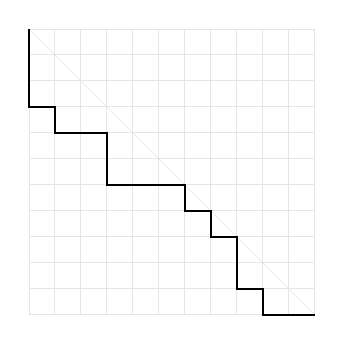
\begin{tikzpicture}[xscale = 0.33,yscale = 0.33]
      \draw[step=1cm,gray!20,very thin] (0,0) grid (11,11);
      \draw[step=1cm,gray!20,very thin] (0,11)--(11,0); \draw[thick]
      (0,11)--(0,8)--(1,8)--(1,7)--(3,7)--(3,5)--(6,5)--(6,4)--(7,4)--(7,3)--(8,3)--(8,1)--(9,1)--(9,0)--(11,0);
    \end{tikzpicture}
  \end{center}\pause
  \begin{itemize}
  \item \(\area(\lambda) = \) number of squares above \(\lambda\) but
    below the path \(\delta\) of alternating S-E steps. \pause
  \item E.g., above \(\area(\lambda) = 10\).
  \end{itemize}
\end{frame}
\begin{frame}
  \frametitle{Shuffle Conjecture}
  \begin{block}{Conjecture (Haglund-Haiman-Loehr-Remmel-Ulyanov, 2005)}
    \[
      \nabla e_n = \sum_{\lambda \in \DP_n} t^{\area(\lambda)}
      q^{\dinv(\lambda)}\omega\Gcal_{\nu(\lambda)}(x;q^{-1}) \,.
    \]
  \end{block}\pause
  \begin{itemize}
  \item \(q=1\), \(\omega\Gcal_{\nu(\lambda)}(x;1) = s_{b_1} \cdots s_{b_n}\)
    where \(b_i =\) number of vertical steps between line and
    \(\lambda\) in column \(i\).\pause
  \item \(\omega\Gcal_{\nu(\lambda)}\) an ``LLT polynomial'' associated to
    \(\lambda\) given as a \(q\)-weight generating function over
    tuples of row SSYTs.\pause
  \item \(\dinv(\lambda) =\) number of balanced hooks.
  \end{itemize}
\end{frame}
\begin{frame}
  \frametitle{dinv}
   \begin{center}
    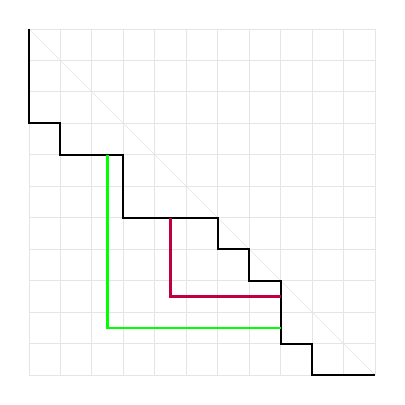
\begin{tikzpicture}[xscale = 0.4,yscale = 0.4]
	\draw[step=1cm,gray!20,very thin] (0,0) grid (11,11);
	\draw[step=1cm,gray!20,very thin] (0,11)--(11,0);
	\draw[thick] (0,11)--(0,8)--(1,8)--(1,7)--(3,7)--(3,5)--(6,5)--(6,4)--(7,4)--(7,3)--(8,3)--(8,1)--(9,1)--(9,0)--(11,0);
        \draw[thick,purple] (4.5,5)--(4.5,2.5)--(8,2.5);
        \draw[thick,green] (2.5,7)--(2.5,1.5)--(8,1.5);
	% \node[left] at (0,10.5) {$1$};
	% \node[left] at (0,9.5) {$3$};
	% \node[left] at (0,8.5) {$4$};
	% \node[left] at (1,7.5) {$1$};
	% \node[left] at (3,6.5) {$3$};
	% \node[left] at (3,5.5) {$5$};
	% \node[left] at (6,4.5) {$2$};
	% \node[left] at (7,3.5) {$1$};
	% \node[left] at (8,2.5) {$1$};
	% \node[left] at (8,1.5) {$6$};
	% \node[left] at (9,0.5) {$4$};
	% \node[left,gray!60] at (11,-0.5) {$1$};
	% \node[left,gray!60] at (10,-0.5) {$2$};
	% \node[left,gray!60] at (9,-0.5) {$3$};
	% \node[left,gray!60] at (8,-0.5) {$4$};
	% \node[left,gray!60] at (7,-0.5) {$5$};
	% \node[left,gray!60] at (6,-0.5) {$6$};
	% \node[left,gray!60] at (5,-0.5) {$7$};
	% \node[left,gray!60] at (4,-0.5) {$8$};
	% \node[left,gray!60] at (3,-0.5) {$9$};
	% \node[left,gray!60] at (2,-0.5) {$10$};
	% \node[left,gray!60] at (1,-0.5) {$11$};
	% \node[left,gray!60] at (0,-0.5) {$j$};
	% \node[left] at (11,-1.5) {$0$};
	% \node[left] at (10,-1.5) {$1$};
	% \node[left] at (9,-1.5) {$1$};
	% \node[left] at (8,-1.5) {$0$};
	% \node[left] at (7,-1.5) {$0$};
	% \node[left] at (6,-1.5) {$0$};
	% \node[left] at (5,-1.5) {$1$};
	% \node[left] at (4,-1.5) {$2$};
	% \node[left] at (3,-1.5) {$1$};
	% \node[left] at (2,-1.5) {$2$};
	% \node[left] at (1,-1.5) {$2$};
	% \node[left] at (0,-1.5) {$c_j$};
	% \node[right,gray!60] at (11.2,11.5){$i$};
	% \node[right,gray!60] at (11.2,10.5){$1$};
	% \node[right,gray!60] at (11.2,9.5) {$2$};
	% \node[right,gray!60] at (11.2,8.5) {$3$};
	% \node[right,gray!60] at (11.2,7.5) {$4$};
	% \node[right,gray!60] at (11.2,6.5) {$5$};
	% \node[right,gray!60] at (11.2,5.5) {$6$};
	% \node[right,gray!60] at (11.2,4.5) {$7$};
	% \node[right,gray!60] at (11.2,3.5) {$8$};
	% \node[right,gray!60] at (11.2,2.5) {$9$};
	% \node[right,gray!60] at (11,1.5) {$10$};
	% \node[right,gray!60] at (11,0.5) {$11$};
	% \node at (14.3,11.5) {$r_i$};
	% \node at (14.2,10.5) {$0$};
	% \node at (14.2,9.5) {$1$};
	% \node at (14.2,8.5) {$2$};
	% \node at (14.2,7.5) {$2$};
	% \node at (14.2,6.5) {$1$};
	% \node at (14.2,5.5) {$2$};
	% \node at (14.2,4.5) {$0$};
	% \node at (14.2,3.5) {$0$};
	% \node at (14.2,2.5) {$0$};
	% \node at (14.2,1.5) {$1$};
	% \node at (14.2,0.5) {$1$};
\end{tikzpicture}
\end{center} 
Balanced hook is given by a cell below \(\lambda\) satisfying \[
  \frac{\ell}{a+1} < 1-\epsilon < \frac{\ell+1}{a}\,.
\]

\end{frame}
\begin{frame}[fragile]
  \frametitle{LLT Polynomials}
  \[
    \Gcal_\nu(x;q^{-1}) = \sum_{T \in \SSYT(\nu)} q^{-i(T)} x^T
  \]
  for \(i(T)\) the number of attacking inversions:\[
     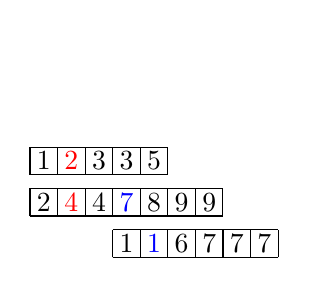
\begin{tikzpicture}[scale=.35]
      \newcounter{c};
      \newcommand{\drawRow}[4]{ \def\r{#1}; \def\a{#2}; \def\b{#3};
        \def\labels{#4}; \draw [shift={(0,1.5*\r)}] (\b+2,1) grid
        (\a+2,0); 
        \setcounter{c}{\a+1}; \foreach
        \nn in \labels {\node at (\thec+2.5,1.5*\r+.5) {
            $\footnotesize \nn$};
          \addtocounter{c}{1}; } };
      \drawRow{2}{0}{5}{1,{\textcolor{red}{2}},3,3,5} \drawRow{1}{0}{7}{2,\textcolor{red}{4},4,\textcolor{blue}{7},8,9,9} \drawRow{0}{3}{9}{1,\textcolor{blue}{1},6,7,7,7}
      % For spacing to center the tableau, not the = sign.
      \node at (8.5,8) {$\,$};
    \end{tikzpicture}
  \]
  \begin{itemize}
  \item \(\Gcal_\nu\) is symmetric and Schur positive.
  \end{itemize}
\end{frame}
% \begin{frame}[fragile]
%   \frametitle{Parking Functions}
%   Label vertical runs decreasing south to north.
%   \begin{center}
%     \begin{tikzpicture}[xscale = 0.4,yscale = 0.4]
% 	\draw[step=1cm,gray!20,very thin] (0,0) grid (11,11);
% 	\draw[step=1cm,gray!20,very thin] (0,11)--(11,0);
% 	\draw[thick] (0,11)--(0,8)--(1,8)--(1,7)--(3,7)--(3,5)--(6,5)--(6,4)--(7,4)--(7,3)--(8,3)--(8,1)--(9,1)--(9,0)--(11,0);
% 	\node[left] at (0,10.5) {$1$};
% 	\node[left] at (0,9.5) {$3$};
% 	\node[left] at (0,8.5) {$4$};
% 	\node[left] at (1,7.5) {$1$};
% 	\node[left] at (3,6.5) {$3$};
% 	\node[left] at (3,5.5) {$5$};
% 	\node[left] at (6,4.5) {$2$};
% 	\node[left] at (7,3.5) {$1$};
% 	\node[left] at (8,2.5) {$1$};
% 	\node[left] at (8,1.5) {$6$};
% 	\node[left] at (9,0.5) {$4$};
% 	% \node[left,gray!60] at (11,-0.5) {$1$};
% 	% \node[left,gray!60] at (10,-0.5) {$2$};
% 	% \node[left,gray!60] at (9,-0.5) {$3$};
% 	% \node[left,gray!60] at (8,-0.5) {$4$};
% 	% \node[left,gray!60] at (7,-0.5) {$5$};
% 	% \node[left,gray!60] at (6,-0.5) {$6$};
% 	% \node[left,gray!60] at (5,-0.5) {$7$};
% 	% \node[left,gray!60] at (4,-0.5) {$8$};
% 	% \node[left,gray!60] at (3,-0.5) {$9$};
% 	% \node[left,gray!60] at (2,-0.5) {$10$};
% 	% \node[left,gray!60] at (1,-0.5) {$11$};
% 	% \node[left,gray!60] at (0,-0.5) {$j$};
% 	% \node[left] at (11,-1.5) {$0$};
% 	% \node[left] at (10,-1.5) {$1$};
% 	% \node[left] at (9,-1.5) {$1$};
% 	% \node[left] at (8,-1.5) {$0$};
% 	% \node[left] at (7,-1.5) {$0$};
% 	% \node[left] at (6,-1.5) {$0$};
% 	% \node[left] at (5,-1.5) {$1$};
% 	% \node[left] at (4,-1.5) {$2$};
% 	% \node[left] at (3,-1.5) {$1$};
% 	% \node[left] at (2,-1.5) {$2$};
% 	% \node[left] at (1,-1.5) {$2$};
% 	% \node[left] at (0,-1.5) {$c_j$};
% 	% \node[right,gray!60] at (11.2,11.5){$i$};
% 	% \node[right,gray!60] at (11.2,10.5){$1$};
% 	% \node[right,gray!60] at (11.2,9.5) {$2$};
% 	% \node[right,gray!60] at (11.2,8.5) {$3$};
% 	% \node[right,gray!60] at (11.2,7.5) {$4$};
% 	% \node[right,gray!60] at (11.2,6.5) {$5$};
% 	% \node[right,gray!60] at (11.2,5.5) {$6$};
% 	% \node[right,gray!60] at (11.2,4.5) {$7$};
% 	% \node[right,gray!60] at (11.2,3.5) {$8$};
% 	% \node[right,gray!60] at (11.2,2.5) {$9$};
% 	% \node[right,gray!60] at (11,1.5) {$10$};
% 	% \node[right,gray!60] at (11,0.5) {$11$};
% 	% \node at (14.3,11.5) {$r_i$};
% 	% \node at (14.2,10.5) {$0$};
% 	% \node at (14.2,9.5) {$1$};
% 	% \node at (14.2,8.5) {$2$};
% 	% \node at (14.2,7.5) {$2$};
% 	% \node at (14.2,6.5) {$1$};
% 	% \node at (14.2,5.5) {$2$};
% 	% \node at (14.2,4.5) {$0$};
% 	% \node at (14.2,3.5) {$0$};
% 	% \node at (14.2,2.5) {$0$};
% 	% \node at (14.2,1.5) {$1$};
% 	% \node at (14.2,0.5) {$1$};
% \end{tikzpicture}
% % \quad
%     % \begin{tikzpicture}[scale=.35]
%     %   \newcounter{c};
%     %   \newcommand{\drawRow}[4]{ \def\r{#1}; \def\a{#2}; \def\b{#3};
%     %     \def\labels{#4}; \draw [shift={(0,1.5*\r)}] (\b+2,1) grid
%     %     (\a+2,0); \node at (\a+1,1.5*\r+.5) {$-\infty$}; \node at
%     %     (\b+2.5,1.5*\r+.5) {$\infty$}; \setcounter{c}{\a+1}; \foreach
%     %     \nn in \labels {\node at (\thec+2.5,1.5*\r+.5) {
%     %         $\footnotesize \nn$};
%     %       \addtocounter{c}{1}; } };
%     %   \drawRow{10}{0}{3}{1,3,4} \drawRow{9}{2}{3}{0}
%     %   \drawRow{8}{2}{2}{} \drawRow{7}{1}{3}{3,5} \drawRow{6}{2}{2}{}
%     %   \drawRow{5}{1}{1}{} \drawRow{4}{0}{1}{2} \drawRow{3}{0}{1}{1}
%     %   \drawRow{2}{0}{2}{0,6} \drawRow{1}{1}{2}{4} \drawRow{0}{1}{1}{}
%     %   % For spacing to center the tableau, not the = sign.
%     %   \node at (8.5,8) {$\,$};
%     % \end{tikzpicture}
% \begin{itemize}
% \item \(x^P = \prod_{\text{labels }i} x_i\)
% \item Statistic \(\dinv\) counting ``inverted'' labels on diagonal or
%   adjacent diagonal.
% \item \(\omega \Gcal_{\nu(\lambda)}(x;q^{-1}) = \sum_{P \in \PF(\lambda)} q^{\dinv(P)} x^P\).
% \end{itemize}
%   \end{center}
% \end{frame}
\begin{frame}
  \frametitle{Shuffle Theorem}
  \begin{block}{Representation Theory: Diagonal Harmonics}
    \(DH_n = \left\{ f \in \Q[x_1,\ldots,x_n,y_1,\ldots,y_n] \st
    \sum_{1 \leq j \leq n} \partial_{x_j}^a \partial_{y_j}^b f(x,y) =
    0 \right\}\)
  \end{block}\pause
  \begin{block}{Symmetric Functions}
    Frobenius characteristic \(\nabla e_n\).
  \end{block}\pause
  \begin{block}{Combinatorics: Shuffle Theorem (Carlsson-Mellit, 2018)}
    \(\nabla e_n = \sum_{\lambda \in \DP_n} t^{\area(\lambda)} q^{\dinv(\lambda)} \omega\Gcal_{\nu(\lambda)}(x;q)\).
  \end{block}
\end{frame}
\begin{frame}
  \frametitle{Outline}
  \begin{enumerate}
  \item Symmetric functions, \(S_n\)-representations, and Frobenius characteristic
  \item Diagonal harmonics and shuffle conjectures
  \item {\bf Stable series approach}
  \item Application: extended Delta conjecture
  \end{enumerate}
\end{frame}
\begin{frame}
  \frametitle{Schiffmann's Elliptic Hall Algebra \(\Ecal\)}
  \begin{itemize}
  \item For every coprime \(m,n \in \Z\), subalgebra \(\sym(X^{m,n})
    \isom \sym\), with relations between them. (Burban-Schiffmann, 2012)\pause
  \item \(\Ecal\) acts on \(\sym\), e.g. \[
      e_k[-MX^{m,1}] \cdot 1 = \nabla^m e_k
    \]\pause
  \end{itemize}
  \begin{block}{Rational Shuffle Conjecture (F. Bergeron, Garsia,
      Sergel Leven, Xin, 2016) (Proved by Mellit, 2016)}
    \[e_k[-MX^{m,n}] \cdot 1 = \sum_\lambda t^{\area(\lambda)}
    q^{\dinv_p(\lambda)} \omega \Gcal_{\nu(\lambda)}(X;q^{-1})\]
  where summation is over all \((kn,km)\)-Dyck paths.
  \end{block}
\end{frame}
\begin{frame}
  \frametitle{Rational Path Combinatorics}
   \begin{center}
    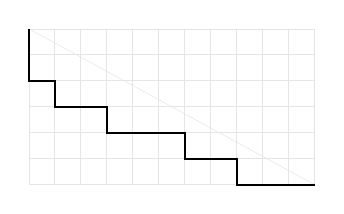
\begin{tikzpicture}[xscale = 0.33,yscale = 0.33]
      \draw[step=1cm,gray!20,very thin] (0,0) grid (11,6);
      \draw[step=1cm,gray!20,very thin] (0,6)--(11,0); \draw[thick]
      (0,6)--(0,4)--(1,4)--(1,3)--(3,3)--(3,2)--(6,2)--(6,1)--(8,1)--(8,0)--(11,0);
    \end{tikzpicture}
  \end{center}\pause
  \begin{itemize}
  \item \(\area(\lambda)\) as before; number of boxes between
    \(\lambda\) and highest path \(\delta\).\pause
  \item \(\dinv_p(\lambda) =\) number of \(p\)-balanced hooks:  \[
    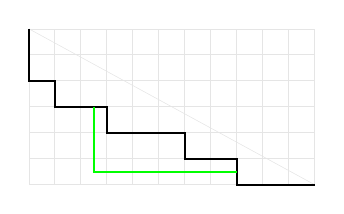
\begin{tikzpicture}[xscale = 0.33,yscale = 0.33]
      \draw[step=1cm,gray!20,very thin] (0,0) grid (11,6);
      \draw[step=1cm,gray!20,very thin] (0,6)--(11,0); \draw[thick]
      (0,6)--(0,4)--(1,4)--(1,3)--(3,3)--(3,2)--(6,2)--(6,1)--(8,1)--(8,0)--(11,0);
      \draw[thick,green] (2.5,3)--(2.5,0.5)--(8,0.5);
    \end{tikzpicture}
      \quad \quad \frac{\ell}{a+1} < p <
      \frac{\ell+1}{a} \quad \quad p = \frac{n}{m}-\epsilon
    \]
  \end{itemize}
\end{frame}
\begin{frame}
  \frametitle{Any Line}
  \begin{block}{Theorem (Blasiak-Haiman-Morse-Pun-S.)}
    Given \(r,s \in \R_{>0}\) such that \(p = s/r\) irrational,
    \pause \[
      D_{(b_1,\ldots,b_l)} \cdot 1 = \sum_{\lambda} t^{\area(\lambda)}
      q^{\dinv_p(\lambda)} \omega \Gcal_{\nu(\lambda)}
    \]\pause
    \begin{itemize}
    \item \(\lambda\) is a lattice path under the line \(y+px=s\),\pause
    \item \((b_1,\ldots,b_l)\) are the south runs of \(\delta\),\pause
    \item \(D_\bb\) is special element of \(\Ecal\).
    \end{itemize}
  \end{block}
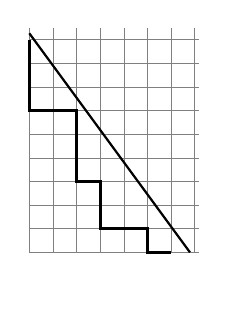
\begin{tikzpicture}[scale=.3, baseline=-.5cm]
\draw[help lines] (0,0) grid (7.2,9.5);
\draw [thick] (0,9.2727) -- (6.8,0);
\draw [very thick] (0,9) -- (0,6) -- (2,6) -- (2,3) -- (3,3) -- (3,1)
-- (5,1) -- (5,0) -- (6,0);
\end{tikzpicture}

\end{frame}
\begin{frame}
  \frametitle{Schiffmann to Shuffle}
  \begin{itemize}
  \item Shuffle algebra \(S\) given by the image of Laurent
    polynomials \(\phi \in \kk[x_1^{\pm 1},\ldots, x_l^{\pm 1}]\) via
    map \pause\[
      H_{q,t}\from \phi \mapsto \sum_{w \in S_l} w \left( \frac{\phi \prod_{i<j}
          (1-qt x_i/x_j)}{\prod_{i<j}((1-x_j/x_i)(1-q x_i/x_j)(1-t x_i/x_j))} \right)
    \]\pause
  \item There exists isomorphism \(\psi \from S \to \Ecal^+\).\pause
  \item (Negut, 2014) gives well-defined \[
    D_{b_1,\ldots,b_l} = \psi \left(H_{q,t}\left(\frac{x_1^{b_1}\cdots
        x_l^{b_l}}{\prod_{i=1}^{l-1} (1-qt x_i/x_{i+1})}  \right)\right)
  \]\pause
  \end{itemize}
  \begin{block}{Key Relationship}
    \[
      \omega(D_\bb \cdot 1)(x_1,\ldots,x_l) = H_{q,t}\left(\frac{x_1^{b_1}\cdots
        x_l^{b_l}}{\prod_{i=1}^{l-1} (1-qt x_i/x_{i+1})}  \right)_{\pol}
    \]
  \end{block}
\end{frame}
\begin{frame}
  \frametitle{Proof Idea}
  \begin{block}{Theorem (Blasiak-Haiman-Morse-Pun-S.)}
    For \(\bb \in \Z^l\) corresponding to some choice of coprime \(m,n\),
    \begin{align*}
&H_{q,t}\left(\frac{x_1^{b_1}\cdots
                     x_l^{b_l}}{\prod_{i=1}^{l-1} (1-qt x_i/x_{i+1})}  \right)\\
      &= \sum_{a_1,\ldots,a_{l-1} \geq 0}
t^{|\aA|} \Lcal^\sigma_{((b_l,\ldots,b_1)+(0,a_{l-1},\ldots,a_1))/(a_{l-1},\ldots,a_1,0)}(x;q)
    \end{align*}
  \end{block}\pause
  \begin{itemize}
  \item Infinite series of \(GL_l\)-characters \(\chi_\lambda\) where
    \(\lambda \in \Z^l\) satisfies \(\lambda_1 \geq \cdots \geq
    \lambda_l\). \pause
  \item \(\chi_\lambda \correspondsto s_\lambda\) when \(\lambda_l \geq 0\).\pause
  \item Under polynomial truncation, \(\Lcal^\sigma_{\beta/\alpha} \to q^{\dinv_p(\lambda)}\Gcal_{\nu(\lambda)}\)
  \end{itemize}
\end{frame}
\begin{frame}
  \frametitle{Cauchy Identity}
  \begin{itemize}
  \item (Twisted) non-symmetric Hall-Littlewood polynomials
    \(E_\lambda^\sigma(x;q)\) defined via Demazure-Lusztig
    operators. \[
      T_i = qs_i+(1-q)\frac{s_i-1}{1-x_{i+1}/x_i}
    \]\pause
  \item Dual basis \(F_\lambda^\sigma\).\pause
    \begin{block}{Cauchy identity}
      \[ \frac{\prod _{i<j} (1 - q\, t\, x_{i} \, y_{j})}{\prod
          _{i\leq j} (1 - t\, x_{i}\, y_{j})} = \sum _{\aA \geq 0}
        t^{|\aA |}\, E^{\sigma }_{\aA }(x_{1},\ldots,x_{l};q^{-1}) \,
        F^{\sigma }_{\aA }(y_{1},\ldots,y_{l};q),
      \]
    \end{block}\pause
  \item \(\Lcal_{\beta/\alpha} = H_q(
    w_0(F_\beta^{\sigma^{-1}}(x;q)
      \ov{E_\alpha^{\sigma^{-1}}(x;q)})) \)
  \end{itemize}
\end{frame}
\begin{frame}
  \frametitle{What have we learned?}
  \begin{block}{Shuffle Theorem for any path}
    \[
    D_\bb \cdot 1
    =
    \sum_{\lambda} t^{\area(\lambda)}
      q^{\dinv_p(\lambda)} \omega \Gcal_{\nu(\lambda)}
    \]    
  \end{block}\pause
  \begin{block}{Stable Shuffle Theorem}
    \vspace{-0.2in}
    \begin{align*}
    &H_q\left(x^{\bb} \frac{\prod_{i+1 < j} (1-qt x_i/x_j)}{\prod_{i<j} (1-t
    x_i/x_j)} \right)\\
    & =
    \sum_{a_1,\ldots,a_{l-1} \geq 0}
      t^{|\aA|}\Lcal^\sigma_{((b_l,\ldots,b_1)+(0,a_{l-1},\ldots,a_1))/(a_{l-1},\ldots,a_1,0)}(x;q) 
    \end{align*}
  \end{block}\pause
  \begin{block}{Cauchy identity}
    \[
 \frac{\prod _{i<j} (1 - q\, t\, x_{i} \, y_{j})}{\prod
    _{i\leq j} (1 - t\, x_{i}\, y_{j})} =
    \sum _{\aA \geq 0}
        t^{|\aA |}\, E^{\sigma }_{\aA }(x_{1},\ldots,x_{l};q^{-1}) \,
        F^{\sigma }_{\aA }(y_{1},\ldots,y_{l};q),
    \] 
  \end{block}
\end{frame}
\begin{frame}
  \frametitle{Outline}
  \begin{enumerate}
  \item Symmetric functions, \(S_n\)-representations, and Frobenius characteristic
  \item {Diagonal harmonics and shuffle conjectures}
  \item {Stable series approach}
  \item {\bf Application: extended Delta conjecture}
  \end{enumerate}
\end{frame}
\begin{frame}
  \frametitle{Another family of symmetric function operators}
  Changing the eigenvalues of Macdonald polynomials:\[
    \Delta_f H_\mu = f[B_\mu]H_\mu \quad \quad \Delta_f' H_\mu = f[B_\mu-1] H_\mu
  \]
  for any \(f \in \sym\) and \(B_\mu = \sum_{(i,j) \in \mu} q^{i-1} t^{j-1}\). (Note
  \(\Delta_{e_{n-1}}' e_n = \nabla e_n\)). \pause
  \begin{block}{Extended Delta Conjecture (Haglund-Remmel-Wilson, 2018)}
    \begin{align*}
      & \Delta_{h_l} \Delta_{e_{k-1}}' e_n =
      \\ & \langle z^{n-k}\rangle
\sum_{\lambda \in \Dyck_{n+l}} \sum_{P\in\LD_{n+l,l}(\lambda)}
q^{\dinv(P)}t^{\area(\lambda)} x^{\wt_+(P)}
\prod_{r_{i}(\lambda)=r_{i-1}(\lambda)+1} \left(1+ z\,
t^{-r_i(\lambda)}\right) \,,
    \end{align*}
  \end{block}
\end{frame}
\begin{frame}
  \frametitle{Delta Combinatorics}
  \begin{center}
    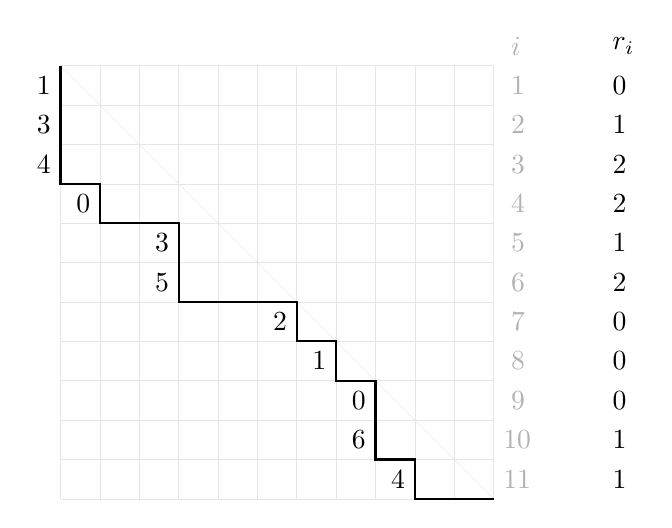
\begin{tikzpicture}[xscale = 0.5,yscale = 0.5]
	\draw[step=1cm,gray!20,very thin] (0,0) grid (11,11);
	\draw[step=1cm,gray!20,very thin] (0,11)--(11,0);
	\draw[thick] (0,11)--(0,8)--(1,8)--(1,7)--(3,7)--(3,5)--(6,5)--(6,4)--(7,4)--(7,3)--(8,3)--(8,1)--(9,1)--(9,0)--(11,0);
	\node[left] at (0,10.5) {$1$};
	\node[left] at (0,9.5) {$3$};
	\node[left] at (0,8.5) {$4$};
	\node[left] at (1,7.5) {$0$};
	\node[left] at (3,6.5) {$3$};
	\node[left] at (3,5.5) {$5$};
	\node[left] at (6,4.5) {$2$};
	\node[left] at (7,3.5) {$1$};
	\node[left] at (8,2.5) {$0$};
	\node[left] at (8,1.5) {$6$};
	\node[left] at (9,0.5) {$4$};
	% \node[left,gray!60] at (11,-0.5) {$1$};
	% \node[left,gray!60] at (10,-0.5) {$2$};
	% \node[left,gray!60] at (9,-0.5) {$3$};
	% \node[left,gray!60] at (8,-0.5) {$4$};
	% \node[left,gray!60] at (7,-0.5) {$5$};
	% \node[left,gray!60] at (6,-0.5) {$6$};
	% \node[left,gray!60] at (5,-0.5) {$7$};
	% \node[left,gray!60] at (4,-0.5) {$8$};
	% \node[left,gray!60] at (3,-0.5) {$9$};
	% \node[left,gray!60] at (2,-0.5) {$10$};
	% \node[left,gray!60] at (1,-0.5) {$11$};
	% \node[left,gray!60] at (0,-0.5) {$j$};
	% \node[left] at (11,-1.5) {$0$};
	% \node[left] at (10,-1.5) {$1$};
	% \node[left] at (9,-1.5) {$1$};
	% \node[left] at (8,-1.5) {$0$};
	% \node[left] at (7,-1.5) {$0$};
	% \node[left] at (6,-1.5) {$0$};
	% \node[left] at (5,-1.5) {$1$};
	% \node[left] at (4,-1.5) {$2$};
	% \node[left] at (3,-1.5) {$1$};
	% \node[left] at (2,-1.5) {$2$};
	% \node[left] at (1,-1.5) {$2$};
	% \node[left] at (0,-1.5) {$c_j$};
	\node[right,gray!60] at (11.2,11.5){$i$};
	\node[right,gray!60] at (11.2,10.5){$1$};
	\node[right,gray!60] at (11.2,9.5) {$2$};
	\node[right,gray!60] at (11.2,8.5) {$3$};
	\node[right,gray!60] at (11.2,7.5) {$4$};
	\node[right,gray!60] at (11.2,6.5) {$5$};
	\node[right,gray!60] at (11.2,5.5) {$6$};
	\node[right,gray!60] at (11.2,4.5) {$7$};
	\node[right,gray!60] at (11.2,3.5) {$8$};
	\node[right,gray!60] at (11.2,2.5) {$9$};
	\node[right,gray!60] at (11,1.5) {$10$};
	\node[right,gray!60] at (11,0.5) {$11$};
	\node at (14.3,11.5) {$r_i$};
	\node at (14.2,10.5) {$0$};
	\node at (14.2,9.5) {$1$};
	\node at (14.2,8.5) {$2$};
	\node at (14.2,7.5) {$2$};
	\node at (14.2,6.5) {$1$};
	\node at (14.2,5.5) {$2$};
	\node at (14.2,4.5) {$0$};
	\node at (14.2,3.5) {$0$};
	\node at (14.2,2.5) {$0$};
	\node at (14.2,1.5) {$1$};
	\node at (14.2,0.5) {$1$};
\end{tikzpicture}
  \end{center}
  \begin{itemize}
  \item Label colums strictly decreasing south to north\pause
  \item \(\wt_+ = x_1^2 x_2 x_3^2 x_4^2 x_5 x_6\)\pause
  \item \(\dinv \correspondsto i(T)\) under suitable translation.
  \end{itemize}
\end{frame}
\begin{frame}
  \frametitle{Application of previous program}
  \begin{block}{Extended Delta Theorem (Blasiak-Haiman-Morse-Pun-S.)}
    \begin{eqnarray*}
      & \bigl( ( h_l[B]e_{k-1}[B-1] e_{n}) \bigr)
      (x_1,\ldots,x_{k+l})\pause \\
      & \displaystyle = \sum_{\substack{s \in \N^{k+r}, |s|=n-k \\ 1 \in J\subset [k+r],
      |J|=k}} \omega \left(D_{s+\varepsilon_J} \cdot 1\right)\pause = \\
      &H_{q,t}\left(
        \frac{ (x_1\cdots
        x_{k+l})}{\prod_{i}(1-qt
      x_i/x_{if1})}h_{n-k}(x_1,\ldots,x_{k+l})\ov{e_l(x_2,\ldots,x_{k+l})}
        \right)_{\pol}\pause\\
      & \displaystyle = \sum_{\substack{J \subset [k+l-1] \\ |J|=l}}
      \sum_{\substack{(0,\aA),\tau \in \N^{k+l} \\ |\tau| = n-k}}
      t^{|\aA|} q^{d(\aA,\tau,J)} (\Lcal_{\beta/\alpha}^{w_0})_{\pol}
    \end{eqnarray*}
  \end{block}
\end{frame}
\begin{frame}
  \frametitle{Stabilizing}
  \begin{block}{Stable Extended Delta Theorem}
    \begin{align*}
      &H_q\left(
        \frac{\prod_{i+1<j} (1-qt x_i/x_j)}{\prod_{i<j}(1-t
      x_i/x_j)}(x_1\cdots
        x_{k+l})h_{n-k}(x_1,\ldots,x_{k+l})\ov{e_l(x_2,\ldots,x_{k+l})}
      \right) \\
      & = \sum_{\substack{J \subset [k+l-1] \\ |J|=l}}
      \sum_{\substack{(0,\aA),\tau \in \N^{k+l} \\ |\tau| = n-k}}
      t^{|\aA|} q^{d(\aA,\tau,J)} \Lcal_{\beta/\alpha}^{w_0}
    \end{align*}
  \end{block}
\end{frame}
\begin{frame}
  \frametitle{What next?}
  \begin{enumerate}
  \item We conjecture \(D_\bb \cdot 1\) is \(q,t\)-Schur positive for
    a broader class of indices.\pause
  \item Combinatorial description of Schur expansion coefficients for
    \(D_\bb \cdot 1\)?\pause
  \item Loehr-Warrington conjecture for \(\nabla s_\lambda\).
  \end{enumerate}
\end{frame}
\begin{frame}[shrink=10]
  \frametitle{References}
  Thank you!
  \begin{bibdiv}
    \begin{biblist}
\bib{MR3556418}{article}{
   author={Bergeron, Francois},
   author={Garsia, Adriano},
   author={Sergel Leven, Emily},
   author={Xin, Guoce},
   title={Compositional $(km,kn)$-shuffle conjectures},
   journal={Int. Math. Res. Not. IMRN},
   date={2016},
   number={14},
   pages={4229--4270},
   issn={1073-7928},
   review={\MR{3556418}},
   doi={10.1093/imrn/rnv272},
}
\bib{paths}{article}{
  author={Blasiak, Jonah},
  author={Haiman, Mark},
  author={Morse, Jennifer},
  author={Pun, Anna},
  author={Seelinger, George H},
  title={A Shuffle Theorem for Paths Under Any Line},
  year={2021},
  journal = {arXiv e-prints},
  eprint={arXiv:2102.07931}
}
\bib{paths}{article}{
  author={Blasiak, Jonah},
  author={Haiman, Mark},
  author={Morse, Jennifer},
  author={Pun, Anna},
  author={Seelinger, George H.},
  title={A proof of the Extended Delta Conjecture},
  year={2021},
  journal = {arXiv e-prints},
  eprint={arXiv:2102.08815}
}
\bib{MR2922373}{article}{
   author={Burban, Igor},
   author={Schiffmann, Olivier},
   title={On the Hall algebra of an elliptic curve, I},
   journal={Duke Math. J.},
   volume={161},
   date={2012},
   number={7},
   pages={1171--1231},
   issn={0012-7094},
   review={\MR{2922373}},
   doi={10.1215/00127094-1593263},
}
\bib{MR3787405}{article}{
   author={Carlsson, Erik},
   author={Mellit, Anton},
   title={A proof of the shuffle conjecture},
   journal={J. Amer. Math. Soc.},
   volume={31},
   date={2018},
   number={3},
   pages={661--697},
   issn={0894-0347},
   review={\MR{3787405}},
   doi={10.1090/jams/893},
}
\bib{MR1214091}{article}{
   author={Garsia, Adriano M.},
   author={Haiman, Mark},
   title={A graded representation model for Macdonald's polynomials},
   journal={Proc. Nat. Acad. Sci. U.S.A.},
   volume={90},
   date={1993},
   number={8},
   pages={3607--3610},
   issn={0027-8424},
   review={\MR{1214091}},
   doi={10.1073/pnas.90.8.3607},
}
\bib{MR2115257}{article}{
    AUTHOR = {Haglund, J. and Haiman, M. and Loehr, N. and Remmel, J. B. and
              Ulyanov, A.},
     TITLE = {A combinatorial formula for the character of the diagonal
              coinvariants},
   JOURNAL = {Duke Math. J.},
  FJOURNAL = {Duke Mathematical Journal},
    VOLUME = {126},
      YEAR = {2005},
    NUMBER = {2},
     PAGES = {195--232},
      ISSN = {0012-7094},
   MRCLASS = {05E10 (05A30 20C30)},
  MRNUMBER = {2115257},
MRREVIEWER = {Edward E. Allen},
       DOI = {10.1215/S0012-7094-04-12621-1},
       URL = {https://doi-org.proxy01.its.virginia.edu/10.1215/S0012-7094-04-12621-1},
}
\bib{MR3811519}{article}{
   author={Haglund, J.},
   author={Remmel, J. B.},
   author={Wilson, A. T.},
   title={The delta conjecture},
   journal={Trans. Amer. Math. Soc.},
   volume={370},
   date={2018},
   number={6},
   pages={4029--4057},
   issn={0002-9947},
   review={\MR{3811519}},
   doi={10.1090/tran/7096},
}
\bib{mellit}{article}{
       author = {{Mellit}, Anton},
        title = {Toric braids and $(m,n)$-parking functions},
      journal = {arXiv e-prints},
     keywords = {Mathematics - Combinatorics, Mathematics - Quantum Algebra, Mathematics - Representation Theory},
         year = {2016},
        month = {apr},
          eid = {arXiv:1604.07456},
        pages = {arXiv:1604.07456},
archivePrefix = {arXiv},
       eprint = {arXiv:1604.07456},
 primaryClass = {math.CO},
}
\bib{MR3283004}{article}{
   author={Negut, Andrei},
   title={The shuffle algebra revisited},
   journal={Int. Math. Res. Not. IMRN},
   date={2014},
   number={22},
   pages={6242--6275},
   issn={1073-7928},
   review={\MR{3283004}},
   doi={10.1093/imrn/rnt156},
}
    \end{biblist}
  \end{bibdiv}
\end{frame}
% \begin{frame}
%   \begin{itemize}
%   \item Define \(\nabla\) by \(\nabla \tilde{H}_\mu = B_\mu(q,t) \tilde{H}_\mu\) for
%     eigenvalue \(B_\mu(q,t) \in \Q[q,t]\). \[
%       \nabla \tilde{H}_{2,1} = qt \tilde{H}_{2,1}
%     \]\pause
% \item \(\hat{M} \to  \nabla e_n\)
%     \begin{block}{Open question}
%       \pause
%       What is the Schur expansion of \(\nabla e_n\)?
%       \pause
%     \end{block}
%     Recover earlier story by taking \(t=0\) and \(y_i = 1\) for all \(y_i\)'s.
%   \end{itemize}
% \end{frame}
\end{document}
%%% Local Variables:
%%% mode: latex
%%% TeX-master: t
%%% End:
